\documentclass{article}
\usepackage[T1]{fontenc}
\usepackage{lmodern}
\usepackage{graphicx}
\usepackage{amsmath,amssymb}
\usepackage[a4paper,margin=2cm]{geometry}
\usepackage[absolute,overlay]{textpos}
\setlength{\TPHorizModule}{1mm}
\setlength{\TPVertModule}{1mm}
\usepackage[indonesian]{babel}
\usepackage{hyperref}
\setlength{\emergencystretch}{2em}
% unit: Halaman 23

\begin{document}

% === Halaman 23 (llm) ===

\begin{itemize}
    \item OTP pernah digunakan oleh mata-mata (\textit{spy}) selama Perang Dunia II
\end{itemize}

\vspace{80mm}

\textcolor{red}{\centering Pejabat eksekutif operasi khusus dari Inggris memperlihatkan syal yang bertuliskan kunci OTP selama PD II}

\vspace{10mm}

\begin{flushright}
\textcolor{red}{Sumber: John H Reif, History of Computing, Duke University}
\end{flushright}

% deskripsi: Foto seorang pria yang memegang selembar kain atau syal yang berisi teks terenkripsi (one-time pad) yang digunakan oleh mata-mata Perang Dunia II.
% bbox normalisasi: [0.1440, 0.2000, 0.5670, 0.8400]
\begin{textblock*}{88.83mm}(30.24mm,59.40mm)
\noindent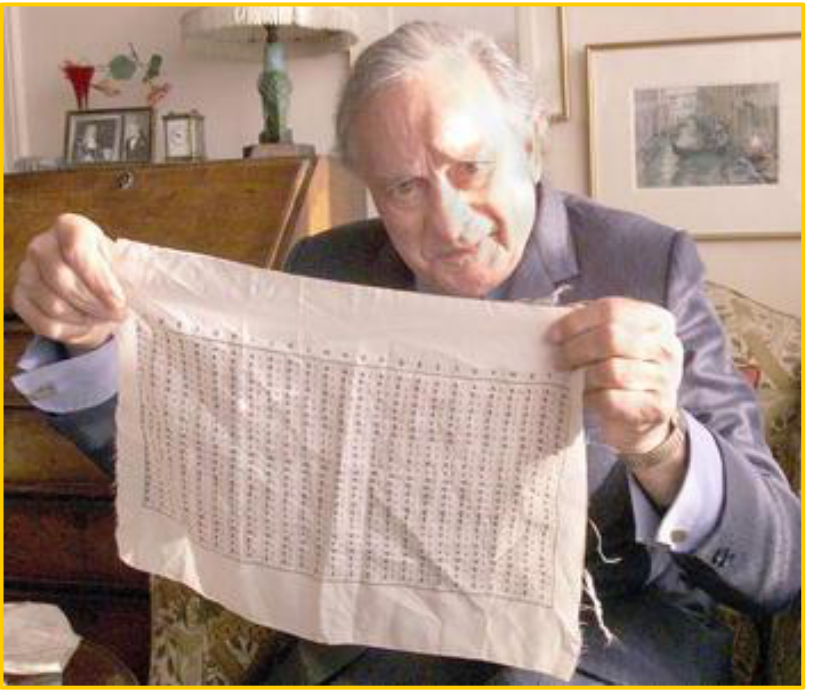
\includegraphics[width=88.83mm,height=190.08mm]{../../images/llm/page_023_img_01.png}%
\end{textblock*}

\end{document}
